\section[Introdução]{Introdução}
Desenvolvido para o \ac{mprs}, o projeto Operações GAECO visa solucionar uma necessidade crítica de integração das aplicações de \ac{mba}, RECUPERA E CUMPRA-SE de forma com que todos os participantes das operações consigam vizualizar os locais, objetos, alvos, entre outras informações e documentá-las.

O processo atual é manual, o que acaba dificultando o acesso das inforamações a todos os integrantes da operação, além não permitir a edição dos documentos, sem precisar refazê-los por completo. Para resolver esse problema, nosso objetivo é desenvolver um aplicativo que permita aos agentes e aos administradores da operação visualizar e criar os alvos e as operações, além de gerar relatórios com um resumo das apreensões.

O projeto, que está sendo desenvolvido durante o segundo semestre de 2025, conta com a orientação do Prof. Rafael Chanin e a colaboração direta dos stakeholders Rovena Zanchet e Frantiele Rodrigues dos Santos. A \autoref{fig:Equipe} mostra o time reunido com o professor e os stakeholders.

\begin{figure}[H]
    \centering
    \small
    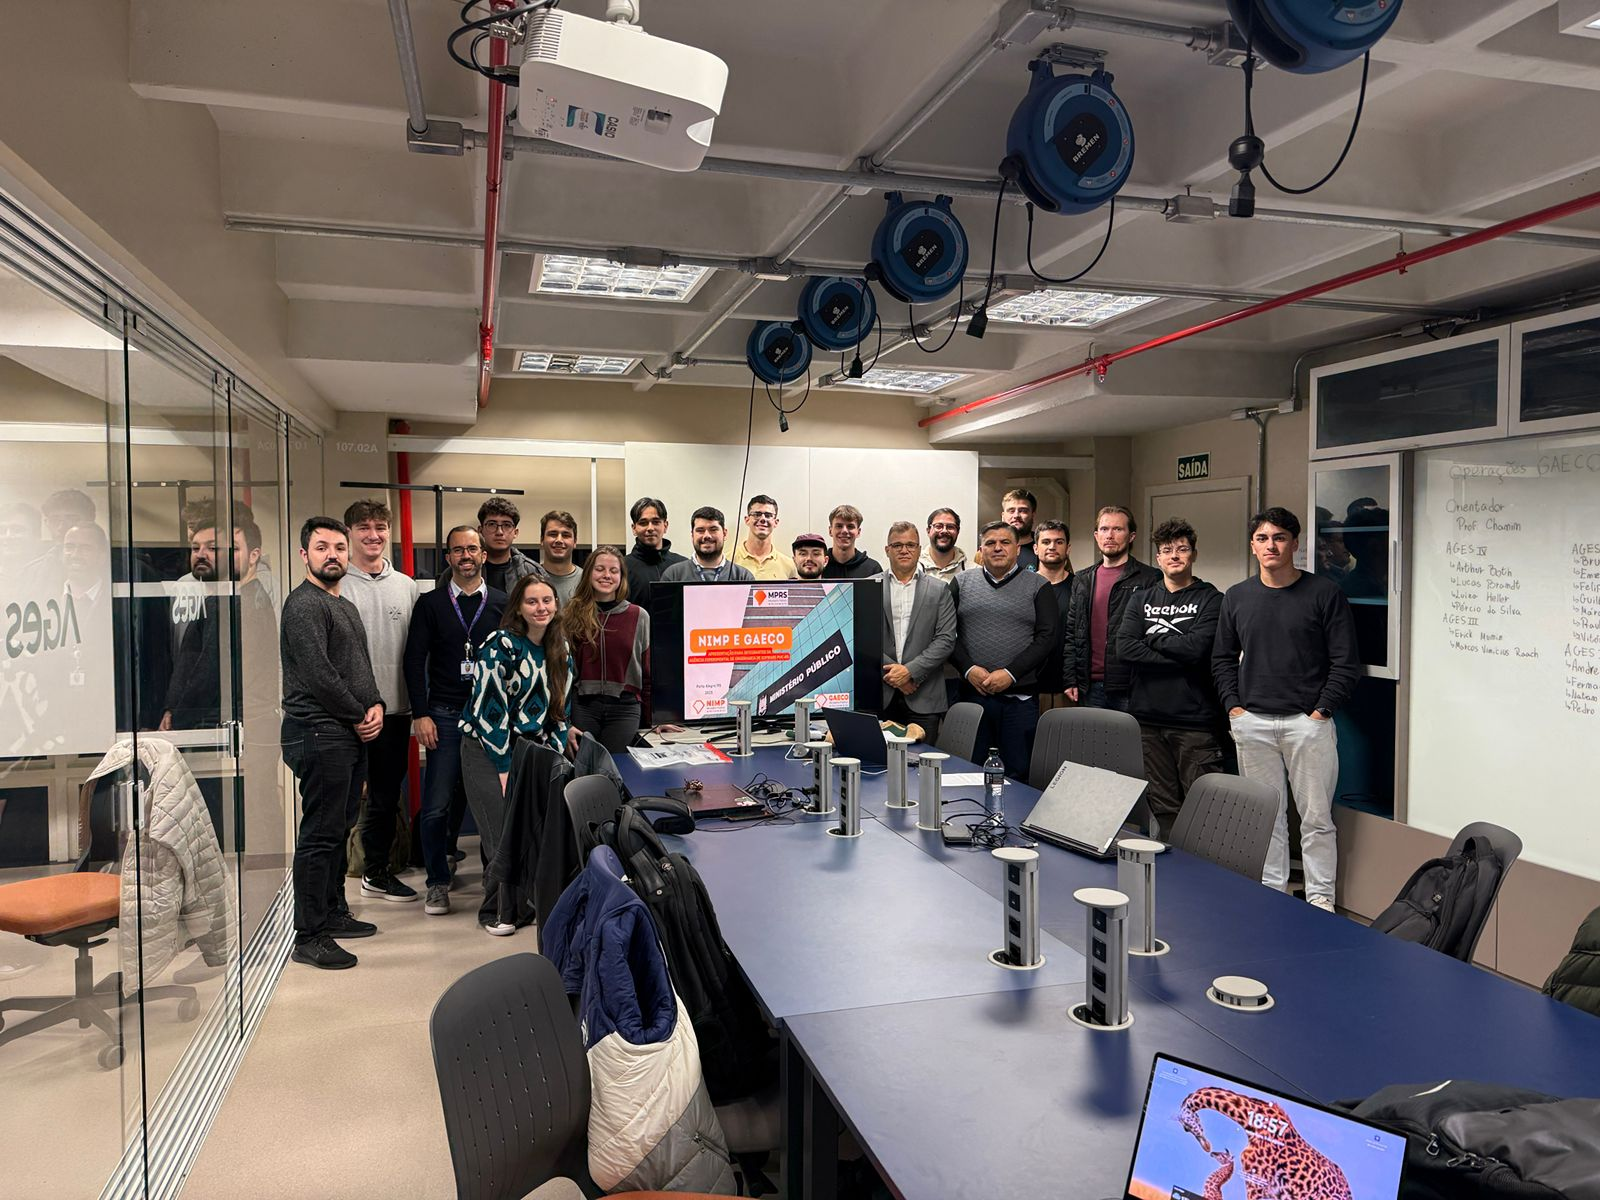
\includegraphics[width=0.7\linewidth]{conteudo//2 - ages I//conteudo//figures//Equipe.jpeg}
    \caption{Time Operações GAECO}
    Fonte: Adaptado de \textcites{wiki-Operacoes GAECO}
    \label{fig:Equipe}
\end{figure}